\documentclass{article}

\usepackage{arxiv}

\usepackage[utf8]{inputenc} % allow utf-8 input
\usepackage[T1]{fontenc}    % use 8-bit T1 fonts
\usepackage{lmodern}        % https://github.com/rstudio/rticles/issues/343
\usepackage{hyperref}       % hyperlinks
\usepackage{url}            % simple URL typesetting
\usepackage{booktabs}       % professional-quality tables
\usepackage{amsfonts}       % blackboard math symbols
\usepackage{nicefrac}       % compact symbols for 1/2, etc.
\usepackage{microtype}      % microtypography
\usepackage{graphicx}

\title{Personal Vehicle Depreciation: Electric vs.~Combustion}

\author{
    Gianluca Van Den Berg
   \\
    Department of Economics \\
    San Francisco State University \\
  San Francisco, CA \\
  \texttt{\href{mailto:gvandenberg@sfsu.edu}{\nolinkurl{gvandenberg@sfsu.edu}}} \\
  }


% tightlist command for lists without linebreak
\providecommand{\tightlist}{%
  \setlength{\itemsep}{0pt}\setlength{\parskip}{0pt}}

% From pandoc table feature
\usepackage{longtable,booktabs,array}
\usepackage{calc} % for calculating minipage widths
% Correct order of tables after \paragraph or \subparagraph
\usepackage{etoolbox}
\makeatletter
\patchcmd\longtable{\par}{\if@noskipsec\mbox{}\fi\par}{}{}
\makeatother
% Allow footnotes in longtable head/foot
\IfFileExists{footnotehyper.sty}{\usepackage{footnotehyper}}{\usepackage{footnote}}
\makesavenoteenv{longtable}

% Pandoc citation processing
\newlength{\cslhangindent}
\setlength{\cslhangindent}{1.5em}
\newlength{\csllabelwidth}
\setlength{\csllabelwidth}{3em}
\newlength{\cslentryspacingunit} % times entry-spacing
\setlength{\cslentryspacingunit}{\parskip}
% for Pandoc 2.8 to 2.10.1
\newenvironment{cslreferences}%
  {}%
  {\par}
% For Pandoc 2.11+
\newenvironment{CSLReferences}[2] % #1 hanging-ident, #2 entry spacing
 {% don't indent paragraphs
  \setlength{\parindent}{0pt}
  % turn on hanging indent if param 1 is 1
  \ifodd #1
  \let\oldpar\par
  \def\par{\hangindent=\cslhangindent\oldpar}
  \fi
  % set entry spacing
  \setlength{\parskip}{#2\cslentryspacingunit}
 }%
 {}
\usepackage{calc}
\newcommand{\CSLBlock}[1]{#1\hfill\break}
\newcommand{\CSLLeftMargin}[1]{\parbox[t]{\csllabelwidth}{#1}}
\newcommand{\CSLRightInline}[1]{\parbox[t]{\linewidth - \csllabelwidth}{#1}\break}
\newcommand{\CSLIndent}[1]{\hspace{\cslhangindent}#1}

\begin{document}
\maketitle


\begin{abstract}

\end{abstract}


\hypertarget{gianluca-vandenberg}{%
\subparagraph{Gianluca Vandenberg}\label{gianluca-vandenberg}}

\hypertarget{id-915219297}{%
\subparagraph{ID: 915219297}\label{id-915219297}}

\hypertarget{section}{%
\subparagraph{12/10/2023}\label{section}}

\hypertarget{introduction}{%
\section{Introduction}\label{introduction}}

Innovation in the automotive industry is required to drive us to a
sustainable future. Electric vehicles are the next step for the industry
to adopt. Removing internal combustion engine (ICE) cars from the road
will help fight climate change, give us cleaner air in metropolitan
areas, and reduce our dependence on fossil fuels.

In recent years, fully electric vehicles (EVs) still only make up about
1\% Blanco (2022) of all cars on the road in the United States. However,
data from recent car sales show that about 8\% of vehicles bought during
Q3 of 203 were electric Automotive (2023). Trends are looking
optimistic, and it will only be a matter of time before EVs become the
vehicles of choice for all Americans.

Owning an EV is different from a traditional gas-powered car in multiple
ways. A costly and heavy battery pack replaces the gas tank, and a
simpler electric motor replaces the complex combustion engine. However,
the heavy battery on the bottom of the vehicle drastically improves
stability, making the car safer. No oil changes are necessary. Besides
the occasional brake inspection and tire change, EVs have little
operating cost compared to their gas-powered counterparts. EV owners
worry about getting to their destination, which makes their `range' a
vital specification when comparing EVs. Then there is the unknown about
the battery's life expectancy and cost of replacement. As technology
quickly evolves in the battery sector, one might fear that their
three-year-old EV will be obsolete soon.

This empirical research seeks to answer the following questions: Q1:
``Do EVs lose more value as the car ages in years than their ICEV
counterparts?''; Q2: ``Do EVs lose more value as the car drives more
miles than their ICEV counterparts?'' The research finds that, on
average, EVs lose marginally more value than gas-powered cars due to
aging. We also find that higher mileage reduces gas-powered car value by
more than double what it does to the value of an EV.

This paper will open with a literature review on depreciation and other
factors influencing EV price economics. Following that, the paper will
highlight the data used and the methodologies used to answer the
research questions. The results and a discussion follow these sections.
The paper will finish with a conclusion, including the limitations of
this paper.

\hypertarget{literature-review}{%
\section{Literature Review}\label{literature-review}}

Addressing the issue of depreciation or value loss for EVs is essential
to be adopted by the general population. There are several reasons why
consumers think it is a bad investment to opt for an EV. Consumers often
view EVs and consumer electronic batteries as similar. Excellent care
will still send the best batteries to the recycling bin within three to
five years. Nevertheless, EV batteries are different and can last much
longer.

Zang, Wang, and Qi (2022) research highlights some interesting facts
about the EV battery. They introduce the idea that measuring an EV's
deprecation by time or millage without considering the battery's
condition is unwise. Given that the battery makes up about 40\% of the
cost of building an EV König et al. (2021), one should include when
determining the amount an EV depreciates. Zang, Wang, and Qi (2022)
identifies the depth-of-discharge (DOD) to significantly impact the
deprecation of the battery, which they mention leads to a naturally
nonlinear depreciation function. DOD refers to the amount a battery uses
(discharges) from the previous charge till it is plugged in again,
unlike conventional car depreciation functions, which see age and
mileage as linear factors. This paper will not be able to use the
battery's condition as a variable. However, this insight makes a case
for adding quadratic terms to find nonlinear trends in the data.

Government intervention plays a role in consumers' consideration of
buying an EV. Incentives such as subsidies, tax breaks, and access to
High-Occupancy Vehicle (HOV) lanes are all meant to entice consumers to
switch to electric driving. In addition to the cost-benefit of lower
operating costs, it is a no-brainer. However, Rapson and Muehlegger
(2023) lists many reasons to think again before committing to the
future. In their paper, Rapson and Muehlegger (2023) mention the lower
range and longer refill times compared to ICEs. Electricity and gas
prices vary widely in the U.S., making charging more expensive than
fueling in certain areas. The only actual maintenance cost of EVs comes
years after purchase when the car needs a new battery, which could cost
up to \$10,000. Compared to the average cost of \$200 annually for ICE
vehicles. The paper mentions that this information is complex to compare
due to the need for historical data on EVs and the potential to reduce
the cost of batteries.

The government intends to reduce carbon emissions by offering financial
incentives to new EV drivers, but Rapson and Muehlegger (2023) states
that the electricity created for EVs is far from clean. Rather than
having carbon dioxide burn right where ICE vehicles drive, EVs send
their greenhouse gas emissions to another place in the country.
Depending on the lifecycle of an EV, they can sometimes pollute more
than traditional cars. The nationwide electricity grid is also
transitioning to green energy and will make EVs much cleaner as this
progresses.

In their research, Breetz and Salon (2018) discusses the necessity for
EV subsidies. As previously mentioned, many factors, including location,
will determine if an EV will be worth the premium price tag. Breetz and
Salon (2018) concluded that EV costs substantially more throughout
five-year ownership in 13 out of 14 cities they analyzed. The biggest
driver of this cost discrepancy is depreciation. The EVs lost more value
in 5 years than they saved in gas and other expenses. This study
analyzed vehicles between 2011 and 2015 with a 24 and 30 kWh capacity
Nissan Leaf, which gives about a 100-mile range. For comparison, the
base Tesla Model 3 had 54 kWh back in 2019.

This paper is similar in research objective and approach in contrast to
Schloter (2022). Both aim to find the comparative depreciation between
EVs and ICEVs. However, MSRP was unavailable in this paper's data,
making it more about the vehicle's expected value than direct
depreciation. Schloter (2022) finds that EVs depreciate substantially
faster than ICEVs. The data they used is from various countries and
mainly aims to demonstrate the depreciation rate over time. This paper
takes a similar approach to find the vehicle's value as they age and
travel further.

\hypertarget{data-overview}{%
\section{Data Overview}\label{data-overview}}

The vehicle sales data used for this research was captured from eBay
over 20 months between 2018 and 2020. The raw data consists of over 120
thousand sales records in the U.S. and Canada. The data provider, a
Kaggle user `tsaustin,' documented Python code that verifies that no
duplicates are present. Since EVs were not a significant part of the
mass passenger vehicle market, vehicles built years prior to 2003 have
no use in the data. Outliers with extremely high or low sales prices,
milages recorded over 150 thousand, and vehicles with insufficient
information are dropped from the data. To avoid including collectible
vehicles, brands with 50 or fewer records in the remaining data set are
also removed.

\hypertarget{table-1}{%
\paragraph{Table 1}\label{table-1}}

\begin{longtable}[]{@{}
  >{\raggedleft\arraybackslash}p{(\columnwidth - 24\tabcolsep) * \real{0.0446}}
  >{\raggedleft\arraybackslash}p{(\columnwidth - 24\tabcolsep) * \real{0.0637}}
  >{\raggedleft\arraybackslash}p{(\columnwidth - 24\tabcolsep) * \real{0.0573}}
  >{\raggedright\arraybackslash}p{(\columnwidth - 24\tabcolsep) * \real{0.0510}}
  >{\raggedleft\arraybackslash}p{(\columnwidth - 24\tabcolsep) * \real{0.0510}}
  >{\raggedright\arraybackslash}p{(\columnwidth - 24\tabcolsep) * \real{0.1146}}
  >{\raggedright\arraybackslash}p{(\columnwidth - 24\tabcolsep) * \real{0.1210}}
  >{\raggedleft\arraybackslash}p{(\columnwidth - 24\tabcolsep) * \real{0.0318}}
  >{\raggedright\arraybackslash}p{(\columnwidth - 24\tabcolsep) * \real{0.0892}}
  >{\raggedright\arraybackslash}p{(\columnwidth - 24\tabcolsep) * \real{0.1529}}
  >{\raggedright\arraybackslash}p{(\columnwidth - 24\tabcolsep) * \real{0.0764}}
  >{\raggedleft\arraybackslash}p{(\columnwidth - 24\tabcolsep) * \real{0.0828}}
  >{\raggedright\arraybackslash}p{(\columnwidth - 24\tabcolsep) * \real{0.0637}}@{}}
\caption{Head of Original Data (source:
\url{https://www.kaggle.com/datasets/tsaustin/us-used-car-sales-data/})}\tabularnewline
\toprule\noalign{}
\begin{minipage}[b]{\linewidth}\raggedleft
ID
\end{minipage} & \begin{minipage}[b]{\linewidth}\raggedleft
pricesold
\end{minipage} & \begin{minipage}[b]{\linewidth}\raggedleft
yearsold
\end{minipage} & \begin{minipage}[b]{\linewidth}\raggedright
zipcode
\end{minipage} & \begin{minipage}[b]{\linewidth}\raggedleft
Mileage
\end{minipage} & \begin{minipage}[b]{\linewidth}\raggedright
Make
\end{minipage} & \begin{minipage}[b]{\linewidth}\raggedright
Model
\end{minipage} & \begin{minipage}[b]{\linewidth}\raggedleft
Year
\end{minipage} & \begin{minipage}[b]{\linewidth}\raggedright
Trim
\end{minipage} & \begin{minipage}[b]{\linewidth}\raggedright
Engine
\end{minipage} & \begin{minipage}[b]{\linewidth}\raggedright
BodyType
\end{minipage} & \begin{minipage}[b]{\linewidth}\raggedleft
NumCylinders
\end{minipage} & \begin{minipage}[b]{\linewidth}\raggedright
DriveType
\end{minipage} \\
\midrule\noalign{}
\endfirsthead
\toprule\noalign{}
\begin{minipage}[b]{\linewidth}\raggedleft
ID
\end{minipage} & \begin{minipage}[b]{\linewidth}\raggedleft
pricesold
\end{minipage} & \begin{minipage}[b]{\linewidth}\raggedleft
yearsold
\end{minipage} & \begin{minipage}[b]{\linewidth}\raggedright
zipcode
\end{minipage} & \begin{minipage}[b]{\linewidth}\raggedleft
Mileage
\end{minipage} & \begin{minipage}[b]{\linewidth}\raggedright
Make
\end{minipage} & \begin{minipage}[b]{\linewidth}\raggedright
Model
\end{minipage} & \begin{minipage}[b]{\linewidth}\raggedleft
Year
\end{minipage} & \begin{minipage}[b]{\linewidth}\raggedright
Trim
\end{minipage} & \begin{minipage}[b]{\linewidth}\raggedright
Engine
\end{minipage} & \begin{minipage}[b]{\linewidth}\raggedright
BodyType
\end{minipage} & \begin{minipage}[b]{\linewidth}\raggedleft
NumCylinders
\end{minipage} & \begin{minipage}[b]{\linewidth}\raggedright
DriveType
\end{minipage} \\
\midrule\noalign{}
\endhead
\bottomrule\noalign{}
\endlastfoot
137178 & 7500 & 2020 & 786** & 84430 & Ford & Mustang & 1988 & LX & 5.0L
Gas V8 & Sedan & 0 & RWD \\
96705 & 15000 & 2019 & 81006 & 0 & Replica/Kit Makes & Jaguar Beck
Lister & 1958 & & 383 Fuel injected & Convertible & 8 & RWD \\
119660 & 8750 & 2020 & 33449 & 55000 & Jaguar & XJS & 1995 & 2+2
Cabriolet & 4.0L In-Line 6 Cylinder & Convertible & 6 & RWD \\
80773 & 11600 & 2019 & 07852 & 97200 & Ford & Mustang & 1968 & Stock &
289 cu. in. V8 & Coupe & 8 & RWD \\
64287 & 44000 & 2019 & 07728 & 40703 & Porsche & 911 & 2002 & Turbo X-50
& 3.6L & Coupe & 6 & AWD \\
132695 & 950 & 2020 & 462** & 71300 & Mercury & Montclair & 1965 & & NO
ENGINE & Sedan & 0 & RWD \\
\end{longtable}

The raw data set includes 13 variables that help identify each vehicle's
`Power By' designation: Electric, Hybrid, and Gas. Gas vehicles refer to
both ICEVs powered by gas and diesel. Once identified, the Hybrid
vehicles are dropped from the data as this research focuses on the
difference between ICEVs and EVs. After filtering out unuseful data, the
number of sales records available for regression is 36,229 for ICEVs and
EVs combined.

\hypertarget{table-2}{%
\paragraph{Table 2}\label{table-2}}

\begin{longtable}[]{@{}lr@{}}
\caption{Summary of Observations}\tabularnewline
\toprule\noalign{}
PowerBy & \# of Vehicles \\
\midrule\noalign{}
\endfirsthead
\toprule\noalign{}
PowerBy & \# of Vehicles \\
\midrule\noalign{}
\endhead
\bottomrule\noalign{}
\endlastfoot
Gas & 35638 \\
Unknown & 3513 \\
Electric & 591 \\
Hybrid & 491 \\
\end{longtable}

The amount of ICEV records is much larger than that of the EVs. It does
not cause any misrepresentation as the ratio between the two types in
the data set is roughly the same as that of passenger vehicles on the
road when the data was collected. Figure 1 shows an evenly distributed
amount of ICEVs for any car age in our range of 0 to 15, whereas the EV
observations decline when they surpass seven years. Why the amount of
observations drops is unclear and will be an interesting question for
future research. Furthermore, Figure 2 shows a similar trend for EVs
with more than 50 thousand miles on the road. It is uncertain from this
data if there is a reliability issue with EVs past these markers, though
this paper will evaluate if EVs are more prone to value loss at these
stages in their lifespan.

\hypertarget{figure-1}{%
\paragraph{Figure 1}\label{figure-1}}

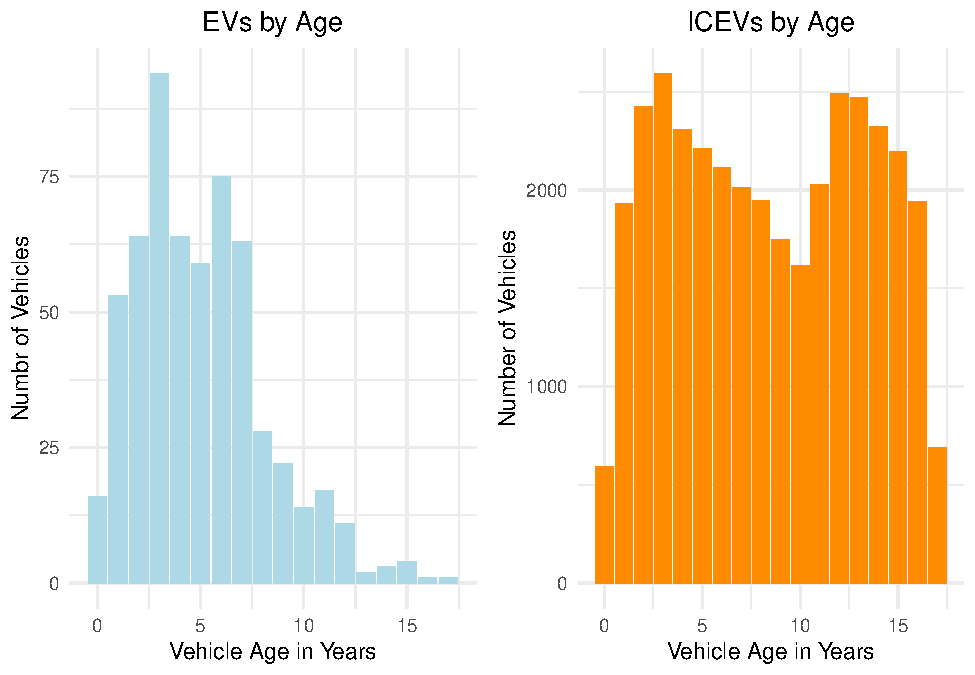
\includegraphics{EV_Project_files/figure-latex/unnamed-chunk-5-1.pdf}

\hypertarget{figure-2}{%
\paragraph{Figure 2}\label{figure-2}}

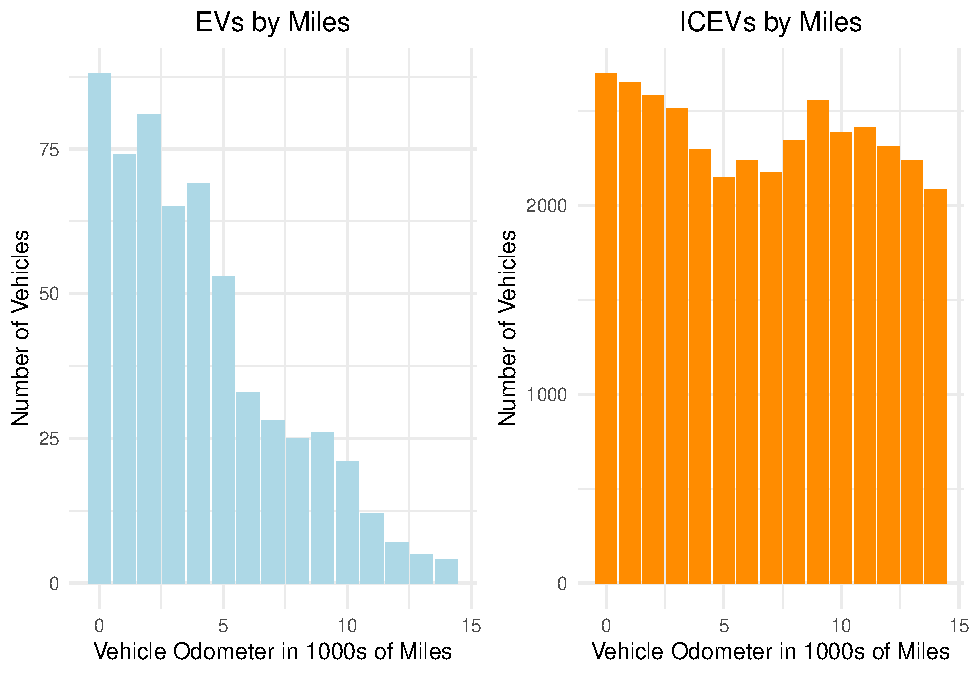
\includegraphics{EV_Project_files/figure-latex/unnamed-chunk-6-1.pdf}

\hypertarget{methodology}{%
\section{Methodology}\label{methodology}}

The regression for this analysis consists of variables to ensure the
highest possible accuracy for the results that will answer the research
questions. The dependent variable for this research is the log function
of `price sold.' Prior research showed a strong correlation between
mileage and car age. This notion holds in this data set. The regression
needs a ratio interaction between the two to avoid any errors resulting
from multicollinearity. Additionally, during the COVID-19 crisis, new
and second-hand vehicles increased in price due to supply chain issues.
The regression includes the year a vehicle was sold as a factor variable
to account for this price shift.

The regression includes dummy variables indicating the vehicle's origin,
domestic, Asia, or Europe, where `domestic' is the omitted variable. The
vehicles' origins are identified by their `Make.' During the
experimentation phase of this research, many `Makes' did not provide
significant results. Collecting them into broader categories improved
the output of the regressions.

`Mileage' and `Car Age' are also regressed as factors to understand
better when depreciation happens. The omitted factor for Mileage is
vehicles driven between 0 and 25K miles. The subsequent factors are
miles 25K to 50K and miles over 50K. During the experimentation, another
factor was added but showed no improvements to the significance of the
results. Car Age is similar, with the lowest age of 0 to 3 years
omitted. The subsequent factors are 4 to 6 years, 7 to 10 years, and
over ten years.

\hypertarget{regression}{%
\paragraph{Regression}\label{regression}}

\[
ln(P_{i})= \beta_{0} + \beta_{1} \cdot  {\frac {M_{i}} {A_{i}}} + \beta_{2} \cdot
Y_{i} + \delta_{1} \cdot O_{asia} + \delta_{2} \cdot O_{euro} + \delta_{3} \cdot M_{25-50}
+ \delta_{4} \cdot M_{50+} + \delta_{5} \cdot A_{4-6} + \delta_{6} \cdot A_{7-10}
+ \delta_{7} \cdot A_{10+}
\]

\(P_{i}\): price of vehicle sold

\(M_{i}\): 1000s miles driven

\(A_{i}\): vehicle age in years

\(Y_{i}\): year the vehicle was sold (factor)

\(O_{asia}\): vehicle origin is Asia (dummy)

\(O_{euro}\): vehicle origin is Europe (dummy)

\(M_{25-50}\): vehicle odometer between 25K \& 50K miles (dummy)

\(M_{50+}\): vehicle odometer over 50K miles (dummy)

\(A_{4-6}\): vehicle age between 4 \& 6 years (dummy)

\(A_{7-10}\): vehicle age between 7 \& 10 years (dummy)

\(A_{4-6}\): vehicle age over 10 years (dummy)

The same regression is run on EVs and ICEVs separately. This way, a
side-by-side comparison can clearly identify differences in the results.
All the previously described variables are added to our linear model and
quantile regression to see which section of the data is mainly affected
by age and mileage.

\hypertarget{results}{%
\section{Results}\label{results}}

The results of the linear model regressions show that most variables
provided significant results. The \(R^2\) for the model on the EV data
set is 0.746, whereas the ICEVs model's \(R^2\) is 0.439. The `Mileage'
over `Car Age' interaction provides little conclusive information other
than a correlation between the two. `Year Sold' provides little
significant data other than the expected increase in price in 2020 for
ICEVs. The EVs give insignificant results, likely due to the small
number of observations relative to those of ICEVs.

The `origin' factor gives a surprising result for European vehicles.
European EVs have a lower price sold than domestic, whereas for ICEVs,
it is the opposite. One explanation can be that domestic EVs, such as
Tesla, are relatively more pricey than domestic ICEVs. Additionally,
Many EVs shipped from overseas tend to be designed for city driving and
are smaller.

To answer Q1, we look at the result of the `Car Age' factors provided at
the bottom. At a glance, it is easy to confirm the consensus that EVs
depreciate quicker as the car ages compared to ICEVs. Only after 10+
years of age have both types of vehicles lost enough value to where they
become close in depreciation.

Right above those results are the Mileage factors. Unfortunately, the
Mileage 25K to 50K shows no significant results compared to the omitted
variable, Mileage 0 to 25K. However, the results for mileage over 50K
tell us that EVs are significantly less affected by miles driven than
ICEVs.

\hypertarget{linear-model-results}{%
\paragraph{Linear Model Results}\label{linear-model-results}}

\begin{verbatim}
## 
## ===========================================================================
##                                       Dependent variable:                  
##                     -------------------------------------------------------
##                                         log(pricesold)                     
##                                EVs                        ICEVs            
##                                (1)                         (2)             
## ---------------------------------------------------------------------------
## I(K_Miles/Car_Age)            0.005                     -0.012***          
##                              (0.006)                     (0.001)           
##                                                                            
## yearsold2019                  0.281                       0.026            
##                              (0.252)                     (0.038)           
##                                                                            
## yearsold2020                  0.284                      0.096**           
##                              (0.253)                     (0.038)           
##                                                                            
## OriginAsia                  -1.430***                   -0.173***          
##                              (0.090)                     (0.010)           
##                                                                            
## OriginEurope                -1.510***                   0.185***           
##                              (0.061)                     (0.009)           
##                                                                            
## Mileage_25Kto50K             -0.0004                    -0.207***          
##                              (0.072)                     (0.015)           
##                                                                            
## Mileage_over50K             -0.294***                   -0.793***          
##                              (0.097)                     (0.018)           
##                                                                            
## Age_4to6                    -0.315***                   -0.075***          
##                              (0.069)                     (0.015)           
##                                                                            
## Age_7to10                   -0.896***                   -0.505***          
##                              (0.091)                     (0.017)           
##                                                                            
## Age_over10                  -0.981***                   -0.943***          
##                              (0.122)                     (0.018)           
##                                                                            
## Constant                    10.400***                   10.200***          
##                              (0.257)                     (0.040)           
##                                                                            
## ---------------------------------------------------------------------------
## Observations                   591                       35,638            
## R2                            0.746                       0.439            
## Adjusted R2                   0.741                       0.439            
## Residual Std. Error     0.559 (df = 580)           0.740 (df = 35627)      
## F Statistic         170.000*** (df = 10; 580) 2,788.000*** (df = 10; 35627)
## ===========================================================================
## Note:                                           *p<0.1; **p<0.05; ***p<0.01
\end{verbatim}

The quantile regressions are run on the traditional three percentiles,
25th, 50th, and 75th, to provide more depth to the results. An
interesting note is that the cheaper vehicles depreciate quicker than
more expensive ones; This holds for both EVs and ICEVs. What differs
from the original linear model is that the depreciation difference
between vehicles in the 75th percentile inverts when they reach age over
10. There, EVs expect to depreciate less than their ICEV counterparts.

The quantile regression results for mileage are similar to the linear
model regression with little variation between the different
percentiles. The only observation is that vehicles in the 75th
percentile tend to be more affected in their price by a higher mileage
(over 50K) than the ones in the 50th or 25th percentile. However, these
numbers are relatively close to each other.

\hypertarget{quantile-regression-results}{%
\paragraph{Quantile Regression
Results}\label{quantile-regression-results}}

\begin{verbatim}
## 
## ==============================================================================
##                                        Dependent variable:                    
##                    -----------------------------------------------------------
##                                          log(pricesold)                       
##                     EV 25th  ICEV 25th  EV 50th  ICEV 50th  EV 75th  ICEV 75th
##                       (1)       (2)       (3)       (4)       (5)       (6)   
## ------------------------------------------------------------------------------
## I(K_Miles/Car_Age)   0.005   -0.010***  -0.001   -0.011***   0.004   -0.011***
##                     (0.004)   (0.001)   (0.004)   (0.001)   (0.005)   (0.001) 
##                                                                               
## yearsold2019         0.146     0.030     0.145     0.047     0.203     0.046  
##                     (1.530)   (0.042)   (0.383)   (0.042)   (0.306)   (0.043) 
##                                                                               
## yearsold2020         0.110    0.105**    0.109   0.113***    0.134    0.102** 
##                     (1.530)   (0.042)   (0.383)   (0.043)   (0.307)   (0.043) 
##                                                                               
## OriginAsia         -1.270*** -0.092*** -1.700*** -0.172*** -1.820*** -0.248***
##                     (0.134)   (0.013)   (0.042)   (0.011)   (0.036)   (0.012) 
##                                                                               
## OriginEurope       -1.560*** 0.245***  -1.790*** 0.170***  -1.900*** 0.104*** 
##                     (0.072)   (0.013)   (0.035)   (0.011)   (0.051)   (0.012) 
##                                                                               
## Mileage_25Kto50K    -0.018   -0.134***  0.069*   -0.203***  -0.052   -0.240***
##                     (0.068)   (0.017)   (0.042)   (0.016)   (0.056)   (0.016) 
##                                                                               
## Mileage_over50K    -0.293**  -0.719*** -0.199*** -0.794*** -0.374*** -0.800***
##                     (0.128)   (0.022)   (0.063)   (0.021)   (0.074)   (0.021) 
##                                                                               
## Age_4to6           -0.391*** -0.164*** -0.234*** -0.038**  -0.216***   0.008  
##                     (0.115)   (0.018)   (0.040)   (0.016)   (0.054)   (0.016) 
##                                                                               
## Age_7to10          -1.080*** -0.639*** -0.707*** -0.474*** -0.547*** -0.380***
##                     (0.143)   (0.021)   (0.077)   (0.019)   (0.063)   (0.020) 
##                                                                               
## Age_over10         -0.921*** -1.160*** -0.750*** -0.916*** -0.540*** -0.728***
##                     (0.162)   (0.022)   (0.096)   (0.021)   (0.116)   (0.021) 
##                                                                               
## Constant           10.400*** 9.780***  10.700*** 10.200*** 10.900*** 10.600***
##                     (1.530)   (0.043)   (0.385)   (0.044)   (0.310)   (0.045) 
##                                                                               
## ------------------------------------------------------------------------------
## Observations          591     35,638      591     35,638      591     35,638  
## ==============================================================================
## Note:                                              *p<0.1; **p<0.05; ***p<0.01
\end{verbatim}

\hypertarget{discussion}{%
\section{Discussion}\label{discussion}}

During the experimental phase, this research created many different
forms of regression to illustrate the difference between EVs' and ICEVs'
depreciation. The literature review helped bring new insight to
answering the research questions. With that insight, the answers to the
following questions were found: Q1: ``Do EVs lose more value as the car
ages in years than their ICEV counterparts?''; Q2: ``Do EVs lose more
value as the car drives more miles than their ICEV counterparts?

To answer Q1, yes, EVs lose more value than ICEVs as the car ages. The
results showed a clear and significant difference of about 24\% from 0-3
to 4-6 years. That difference increased as we compare 0-3 to 7-10 years
but quickly reverses to only 4\% more in value loss for EVs over ten
years.

The answer to Q2 is no; EVs retain more value than ICEVs as the car
increases mileage. Also, these numbers are significant when comparing
0-25K miles to those over 50K miles; EVs lose, on average, 29\% of
value, keeping everything else constant, whereas ICEVs lose 79\%.

\hypertarget{conclusion}{%
\section{Conclusion}\label{conclusion}}

This paper seeks to find out why and if EVs lose more value than ICEVs.
This is an important question for future buyers who will help reduce
dependency on fossil fuels and improve air quality. Literature has
suggested that car age does play a significant role in the depreciation
disparity, yet mileage has received little attention. The literature
also highlighted some limitations of this paper, mainly the need for
more information on (changing) state subsidies and EV battery
conditions.

The data set provided a wide range of vehicle types, build years, and
mileages. Many older vehicles are eliminated to create two comparable
data sets between EVs and ICEVs. The regression, with the dependent
variable log of `price sold,' comprises various independent variables to
account for external factors outside the research questions influencing
the vehicle price sold.

On average, EVs lose more value than ICEVs as they age, ceteris paribus.
Nevertheless, ICEVs lose more value on average than EVs as more miles
are put on the vehicle, ceteris paribus. One unfortunate limitation is
that the \(R^2\) value of the ICEV linear regression is 0.439. Unlike
social science questions, this research would expect a better fit with
this data. It is likely that unaccounted variables such as car color,
location, engine size, vehicle type, and MSRP cause the low \(R^2\)
value. Many of these variables are a considerable chunk that determines
the value of a vehicle.

This research highlights the need for more understanding of proper EV
valuation. Future analysis should include battery condition and a
predictor of battery technology improvement. High improvement in battery
technology can significantly reduce the price and increase the range of
replacement batteries. EV companies should promote the knowledge that
their vehicles depreciate less when driving more miles. However, other
researchers need to further examine this newfound knowledge in greater
detail.

\hypertarget{references}{%
\section*{References}\label{references}}
\addcontentsline{toc}{section}{References}

\hypertarget{refs}{}
\begin{CSLReferences}{1}{0}
\leavevmode\vadjust pre{\hypertarget{ref-coxautoinc}{}}%
Automotive, Cox. 2023. {``Another Quarter, Another Record: EV Sales in
the u.s. Surpass 300,000 in Q3, as Tesla Share of EV Segment Tumbles to
50\%.''} 2023.
\url{https://www.coxautoinc.com/market-insights/q3-2023-ev-sales/}.

\leavevmode\vadjust pre{\hypertarget{ref-caranddriver}{}}%
Blanco, Sebastian. 2022. {``Electric Cars' Turning Point May Be
Happening as u.s. Sales Numbers Start to Climb.''} 2022.
\url{https://www.caranddriver.com/news/a39998609/percentage-of-electric-cars-usa/}.

\leavevmode\vadjust pre{\hypertarget{ref-breetz2018electric}{}}%
Breetz, Hanna L, and Deborah Salon. 2018. {``Do Electric Vehicles Need
Subsidies? Ownership Costs for Conventional, Hybrid, and Electric
Vehicles in 14 US Cities.''} \emph{Energy Policy} 120: 238--49.

\leavevmode\vadjust pre{\hypertarget{ref-konig2021overview}{}}%
König, Adrian, Lorenzo Nicoletti, Daniel Schröder, Sebastian Wolff, Adam
Waclaw, and Markus Lienkamp. 2021. {``An Overview of Parameter and Cost
for Battery Electric Vehicles.''} \emph{World Electric Vehicle Journal}
12 (1): 21.

\leavevmode\vadjust pre{\hypertarget{ref-rapson2023economics}{}}%
Rapson, David S, and Erich Muehlegger. 2023. {``The Economics of
Electric Vehicles.''} \emph{Review of Environmental Economics and
Policy} 17 (2): 274--94.

\leavevmode\vadjust pre{\hypertarget{ref-schloter2022empirical}{}}%
Schloter, Lukas. 2022. {``Empirical Analysis of the Depreciation of
Electric Vehicles Compared to Gasoline Vehicles.''} \emph{Transport
Policy} 126: 268--79.

\leavevmode\vadjust pre{\hypertarget{ref-zang2022column}{}}%
Zang, Yongsen, Meiqin Wang, and Mingyao Qi. 2022. {``A Column Generation
Tailored to Electric Vehicle Routing Problem with Nonlinear Battery
Depreciation.''} \emph{Computers \& Operations Research} 137: 105527.

\end{CSLReferences}

\bibliographystyle{unsrt}
\bibliography{references.bib}


\end{document}
